\documentclass{beamer}

\mode<presentation> {

%\usetheme{default}
%\usetheme{AnnArbor}
%\usetheme{Antibes}
%\usetheme{Bergen}
%\usetheme{Berkeley}
%\usetheme{Berlin}
%\usetheme{Boadilla}
%\usetheme{CambridgeUS}
%\usetheme{Copenhagen}
%\usetheme{Darmstadt}
%\usetheme{Dresden}
%\usetheme{Frankfurt}
%\usetheme{Goettingen}
%\usetheme{Hannover}
%\usetheme{Ilmenau}
%\usetheme{JuanLesPins}
%\usetheme{Luebeck}
\usetheme{Madrid}
%\usetheme{Malmoe}
%\usetheme{Marburg}
%\usetheme{Montpellier}
%\usetheme{PaloAlto}
%\usetheme{Pittsburgh}
%\usetheme{Rochester}
%\usetheme{Singapore}
%\usetheme{Szeged}
%\usetheme{Warsaw}


%\usecolortheme{albatross}
%\usecolortheme{beaver}
%\usecolortheme{beetle}
%\usecolortheme{crane}
%\usecolortheme{dolphin}
%\usecolortheme{dove}
%\usecolortheme{fly}
%\usecolortheme{lily}
%\usecolortheme{orchid}
%\usecolortheme{rose}
%\usecolortheme{seagull}
%\usecolortheme{seahorse}
%\usecolortheme{whale}
%\usecolortheme{wolverine}

%\setbeamertemplate{footline} % To remove the footer line in all slides uncomment this line
%\setbeamertemplate{footline}[page number] % To replace the footer line in all slides with a simple slide count uncomment this line

%\setbeamertemplate{navigation symbols}{} % To remove the navigation symbols from the bottom of all slides uncomment this line
}

\usepackage{graphicx} % Allows including images
\usepackage{booktabs} % Allows the use of \toprule, \midrule and \bottomrule in tables
\usepackage{amsfonts}
\usepackage{mathrsfs}
\usepackage{amsmath,amssymb,graphicx}

%----------------------------------------------------------------------------------------
%	TITLE PAGE
%----------------------------------------------------------------------------------------

\title["7.2"]{7.2: GARCH Models} 

\author{Taylor} 
\institute[UVA] 
{
University of Virginia \\
\medskip
\textit{} 
}
\date{} 

\begin{document}
%----------------------------------------------------------------------------------------

\begin{frame}
\titlepage 
\end{frame}
%----------------------------------------------------------------------------------------

\begin{frame}
\frametitle{Definitions}

Recall the ARCH(p) model (Engle 1982)
\begin{block}{ARCH(p)}
\begin{align*}
Z_t &= \sqrt{h_t}e_t, \hspace{10mm} \{e_t\} \sim IID(0,1) \\
h_t &= \alpha_0 + \sum_{i=1}^p \alpha_i Z^2_{t-i}.
\end{align*}
$\alpha_0 > 0$, $a_i \ge 0$, $p \in \mathbb{N}$
\end{block}


\end{frame}

%----------------------------------------------------------------------------------------

\begin{frame}
\frametitle{A recursive formula}

In the case of ARCH(1), $h_t = \alpha_0 + \alpha_1 Z_{t-1}^2$ and
\begin{align*}
Z_t^2 &= h_t e_t^2\\
&= [\alpha_0 + \alpha_1 Z^2_{t-1}] e_t^2 \\
&= \alpha_0 e_t^2 + \alpha_1 h_{t-1} e_{t-1}^2 e_t^2 \\
&= \alpha_0 e_t^2 + \alpha_1 [\alpha_0 + \alpha_1 Z_{t-2}^2] e_{t-1}^2 e_t^2 \\
&= \alpha_0 e_t^2 + \alpha_1 \alpha_0e_{t-1}^2 e_t^2 + \alpha_1^2 Z_{t-2}^2 e_{t-1}^2 e_t^2 \\
&= \alpha_0 e_t^2 + \alpha_1 \alpha_0e_{t-1}^2 e_t^2 + \alpha_1^2 [h_{t-2}e_{t-2}^2] e_{t-1}^2 e_t^2 \\
&= \alpha_0 e_t^2 + \alpha_1 \alpha_0e_{t-1}^2 e_t^2 + \alpha_1^2 [\alpha_0 + \alpha_1 Z_{t-3}^2 ] e_{t-2}^2 e_{t-1}^2 e_t^2 \\
&=  \left\{\alpha_0 e_t^2 + \alpha_1 \alpha_0e_{t-1}^2 e_t^2  + \alpha_1^2 \alpha_0 e_{t-2}^2 e_{t-1}^2 e_t^2\right\} + \left\{\alpha_1^3  Z_{t-3}^2 e_{t-2}^2 e_{t-1}^2 e_t^2 \right\} \\
&= \alpha_0 \sum_{j=0}^n \alpha_1^j e_t^2 e_{t-1}^2 \cdots e_{t-j}^2 + a_1^{n+1}Z_{t-n-1}^2 e_t^2 e_{t-1}^2 \cdots e_{t-n}^2
\end{align*}


\end{frame}

%----------------------------------------------------------------------------------------

\begin{frame}
\frametitle{A recursive formula}

 
\[
Z_t^2 = \left( \alpha_0 \sum_{j=0}^n \alpha_1^j e_t^2 e_{t-1}^2 \cdots e_{t-j}^2\right) + \left(a_1^{n+1}Z_{t-n-1}^2 e_t^2 e_{t-1}^2 \cdots e_{t-n}^2\right)
\]
If $\alpha_1 < 1$:
\begin{itemize}
\item second term goes to $0$ as $n \to \infty$
\item first term has a limit, let's call it $\alpha_0 \sum_{j=0}^{\infty}\alpha_1^j (e_t^2 \times \cdots \times e_{t-j}^2)$
\end{itemize}
so
\begin{block}{}
\[
Z_t^2 = \alpha_0 \sum_{j=0}^{\infty} \alpha_1^j e_t^2 e_{t-1}^2 \cdots e_{t-j}^2
\]
\end{block}
if we're looking at an infinitely long sequence.
\end{frame}




%----------------------------------------------------------------------------------------

\begin{frame}
\frametitle{Weak-Stationarity}

Weakly-stationary!

\[
E[Z_t] = E[\sqrt{h_t}e_t] = E[\sqrt{h_t}]E[e_t] = 0
\]
Marginal variance
\begin{align*}
\text{Var}[Z_t] &= E[Z_t^2] \\
&= E[\alpha_0 \sum_{j=0}^{\infty} \alpha_1^j e_t^2 e_{t-1}^2 \cdots e_{t-j}^2] \tag{previous slide}\\
&= \alpha_0 \sum_{j=0}^{\infty} \alpha_1^j = \alpha_0/(1-\alpha_1) \tag{linearity, independence, geom. series}
\end{align*}
Autocovariance
\begin{align*}
\gamma_Z(h) &= E[Z_{t+h}Z_t] = E[E(Z_{t+h}Z_t| e_s, s < t+h)] \tag{LTE} \\
&= E[Z_t E(Z_{t+h}| e_s, s < t+h)] = 0
\end{align*}


\end{frame}

%----------------------------------------------------------------------------------------

\begin{frame}
\frametitle{A recursive formula}

But remember that volatility is the {\bf conditional} variance. After taking the square root on both sides of a previous formula

\begin{block}{}
\[
Z_t = e_t \sqrt{\alpha_0\left(1 +  \sum_{j=1}^{\infty} \alpha_1^j e_{t-1}^2 \cdots e_{t-j}^2\right) }.
\]
\end{block}
More recent errors get higher weights in the conditional standard deviation term.
\newline

Also note the small typo in the book.

\end{frame}

%----------------------------------------------------------------------------------------

\begin{frame}
\frametitle{White but not IID}

The ARCH model is white noise, but not IID noise. 

\begin{align*}
E[Z_t^2|Z_{1:t-1}] &= E[(\alpha_0 + \alpha_1 Z_{t-1}^2)e_t^2|Z_{1:t-1}] \\
&= (\alpha_0 + \alpha_1 Z_{t-1}^2) E[e_t^2|Z_{1:t-1}]\\
&= (\alpha_0 + \alpha_1 Z_{t-1}^2) \\
&\neq E[Z_t^2] = \alpha_0 / (1- \alpha_1)
\end{align*}

fun facts:
\begin{itemize}
\item $\{Z_t\}$ cannot be jointly Gaussian (write down the likelihood and it will factor)
\item However it can be conditionally Gaussian (next slide)
\item $Z_t \overset{d}{=} -Z_t$ (previous slide)
\end{itemize}

\end{frame}

%----------------------------------------------------------------------------------------

\begin{frame}
\frametitle{The Conditional Likelihood}

Let's write down the conditional likelihood:
\begin{align*}
L &= f(z_n, z_{n-1},\ldots,z_2 |z_1) \\
&= \prod_{t=2}^n f(z_t|z_{1:t-1}) \\
&= \prod_{t=2}^n \frac{1}{\sqrt{2 \pi h_t } } \exp\left[- \frac{z_t^2}{2 h_t } \right] \tag{cndtl nrmlty} \\ 
&= \prod_{t=2}^n \frac{1}{\sqrt{2 \pi (\alpha_0 + \alpha_1 z_{t-1}^2) } } \exp\left[- \frac{z_t^2}{2(\alpha_0 + \alpha_1 z_{t-1}^2)  } \right] \tag{defn. $h_t$}
\end{align*}

\end{frame}

%----------------------------------------------------------------------------------------

\begin{frame}[fragile]
\frametitle{Test}

Fake data or real data?
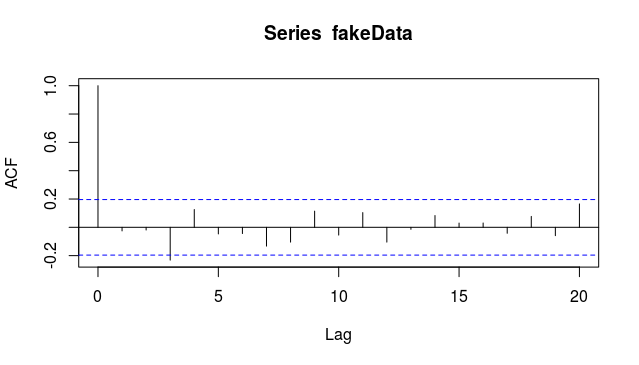
\includegraphics[width=40mm]{/home/taylor/UVa/all_teaching/4170_slides/7/pics/Rplot01.png}
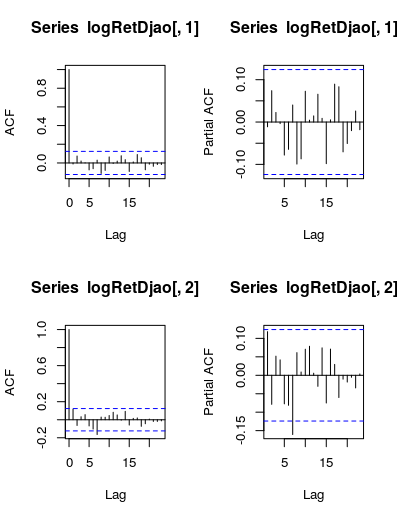
\includegraphics[width=40mm]{/home/taylor/UVa/all_teaching/4170_slides/7/pics/Rplot02.png}
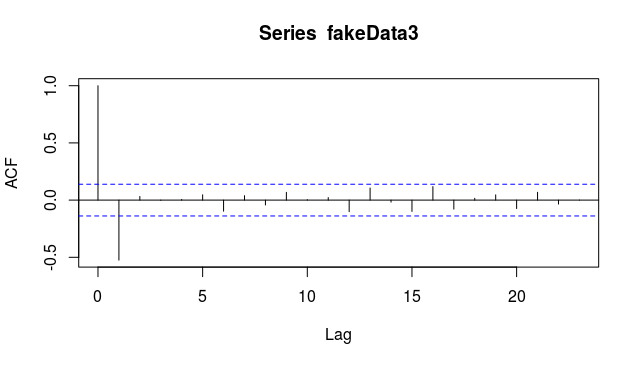
\includegraphics[width=40mm]{/home/taylor/UVa/all_teaching/4170_slides/7/pics/Rplot05.png}
\pause

\begin{verbatim}
spec = garchSpec(model = list(omega = 1, alpha = c(0.5), 
                  beta = 0))
zt <- garchSim(spec, n = 1000)
\end{verbatim}


\end{frame}

%----------------------------------------------------------------------------------------

\begin{frame}[fragile]
\frametitle{Test}

Fake data or real data?
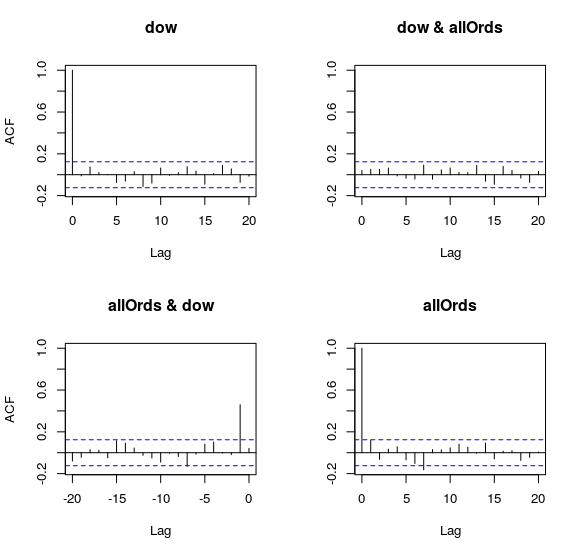
\includegraphics[width=40mm]{/home/taylor/UVa/all_teaching/4170_slides/7/pics/Rplot03.png}
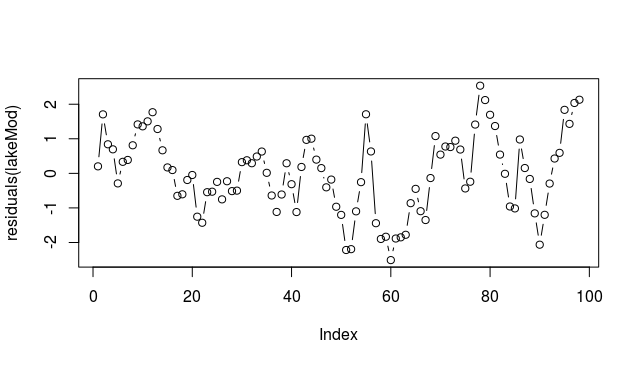
\includegraphics[width=40mm]{/home/taylor/UVa/all_teaching/4170_slides/7/pics/Rplot04.png}
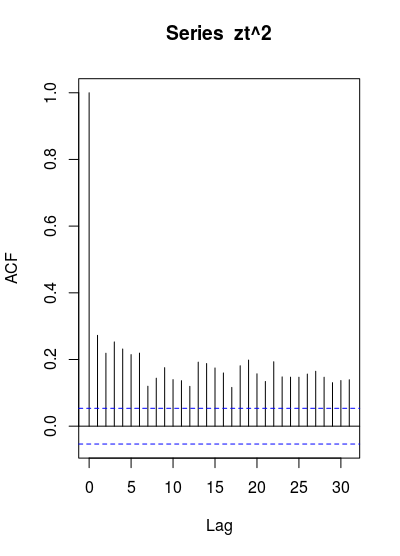
\includegraphics[width=40mm]{/home/taylor/UVa/all_teaching/4170_slides/7/pics/Rplot06.png}
\pause

\begin{verbatim}
getSymbols(Symbols="CVX", src="google")
cvx <- CVX["2012-01-01/2017-04-28"] #remove some of the early stuff
adCVX <- Cl(cvx)
rets <- periodReturn(adCVX, period="daily", type = "log")
\end{verbatim}


\end{frame}

%----------------------------------------------------------------------------------------

\begin{frame}[fragile]
\frametitle{GARCH Models}

Recall the GARCH(p,q) model has the volatility as  
\[
h_t = \alpha_0 + \sum_{i=1}^p \alpha_i Z^2_{t-i} + \sum_{j=1}^q \beta_j h_{t-j},
\]
where $\alpha_0 > 0$, $a_i \ge 0$, $\beta_j \ge 0$, $p \in \mathbb{N}$. This allows for autocorrelation in $h_t$  (clustering).

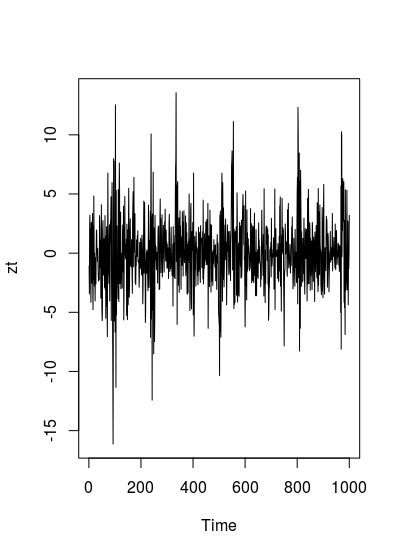
\includegraphics[width=40mm]{/home/taylor/UVa/all_teaching/4170_slides/7/pics/Rplot07.png}
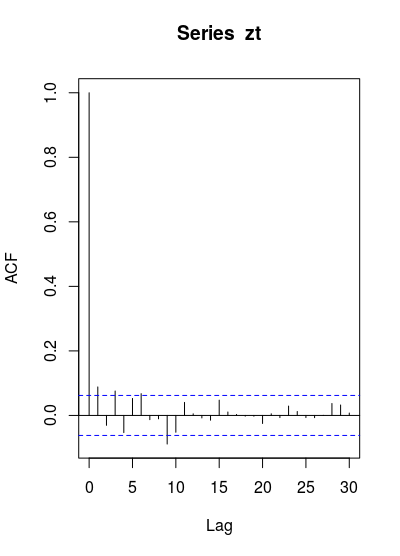
\includegraphics[width=40mm]{/home/taylor/UVa/all_teaching/4170_slides/7/pics/Rplot08.png}
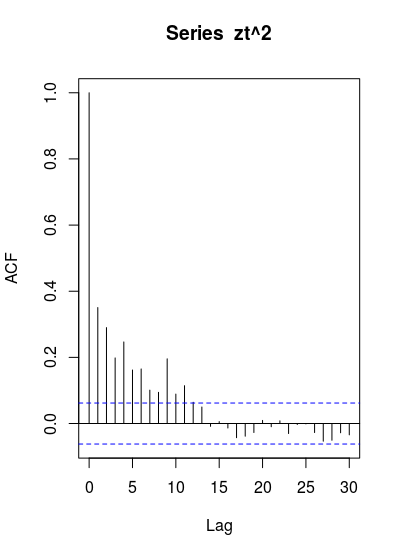
\includegraphics[width=40mm]{/home/taylor/UVa/all_teaching/4170_slides/7/pics/Rplot09.png}


\end{frame}

%----------------------------------------------------------------------------------------

\begin{frame}[fragile]
\frametitle{Example 7.2.2}

See 7.2.R for details. These are the observed returns along with 2 std.dev prediction intervals.

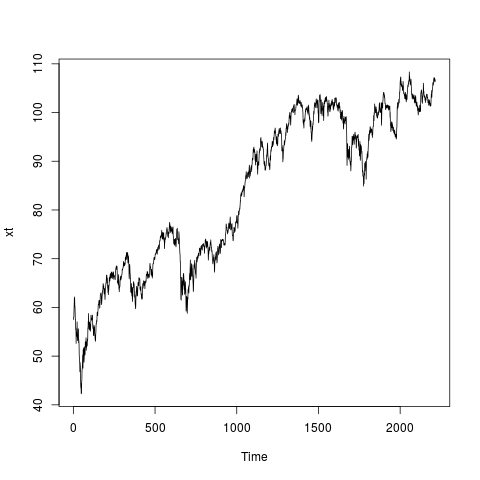
\includegraphics[width=70mm]{/home/taylor/UVa/all_teaching/4170_slides/7/pics/Rplot.png}


\end{frame}

%----------------------------------------------------------------------------------------

\begin{frame}
\frametitle{The Conditional Likelihood}

Sometimes a better fit can be obtained by using t distributions for the conditional likelihood. We assume that $\sqrt{\frac{\nu}{\nu - 2}}e_t \sim t_{\nu}$ with $\nu > 2$. The conditional likelihood:
\begin{align*}
L &= f(z_n, z_{n-1},\ldots,z_2 |z_1) \\
&= \prod_{t=2}^n f(z_t|z_{1:t-1}) \\
&= \prod_{t=2}^n \frac{\Gamma(\frac{\nu+1}{2}) }{\Gamma(\frac{\nu}{2})\Gamma(\frac{1}{2})\sqrt{\nu-2} } \left(1 +\frac{e_t^2 }{\nu-2}  \right)^{- \frac{\nu+1}{2}}
\end{align*}

\end{frame}

%----------------------------------------------------------------------------------------

\begin{frame}[fragile]
\frametitle{Example 7.2.2}

The t distribution fit has a better AIC!

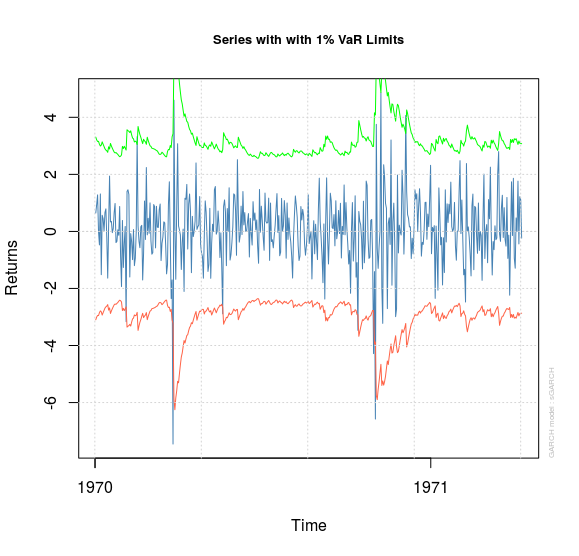
\includegraphics[width=55mm]{/home/taylor/UVa/all_teaching/4170_slides/7/pics/Rplot10.png}

\begin{verbatim}
> (-2*likelihood(fit3))/length(xt)+2*(length(fit3@fit$coef))/length(xt)
[1] 3.094884
> (-2*likelihood(fit))/length(xt)+2*(length(fit@fit$coef))/length(xt)
[1] 3.160894
\end{verbatim}
\end{frame}

%----------------------------------------------------------------------------------------

\begin{frame}[fragile]
\frametitle{Example 7.2.2}

Another example ARIMA(1,1) + GARCH(1,1): 
\[
X_t - \mu = \phi(X_{t-1} - \mu) + Z_t + \theta Z_{t-1} 
\]
\[
Z_t = \sqrt{h_{t}}e_t
\]
\[
h_t = \alpha_0 + \alpha_1 Z_{t-1}^2 + \beta_1 h_{t-1}
\]

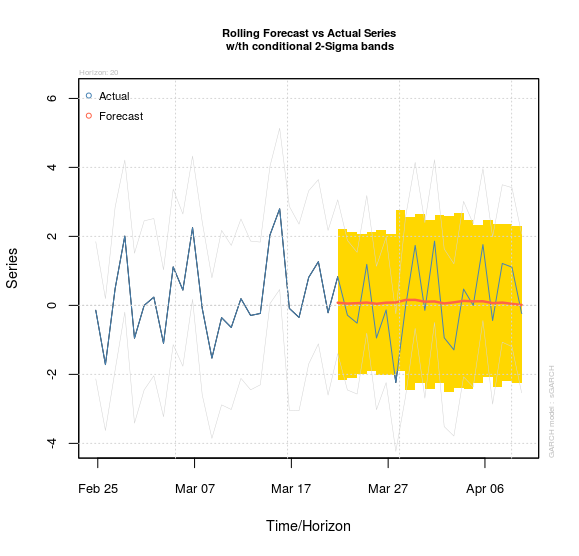
\includegraphics[width=55mm]{/home/taylor/UVa/all_teaching/4170_slides/7/pics/Rplot11.png}
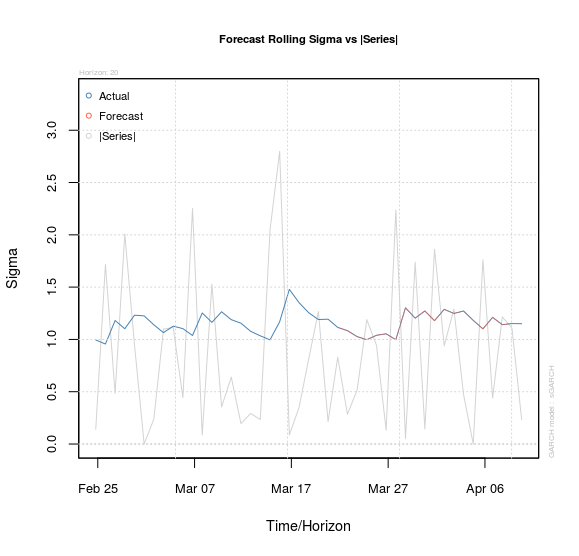
\includegraphics[width=55mm]{/home/taylor/UVa/all_teaching/4170_slides/7/pics/Rplot12.png}

\end{frame}



\end{document} 